\chapter{Altera Cyclone V SoC}
\label{kap:alteracyclone}
The corporation Altera was founded in 1983 and developed its first FPGA in 1992.\cite{althist16} The Altera Cyclone V was developed to decrease time-to-market and cost requirements, simultaneously the power consumption was decreased. Cyclone V devices are made in 28 nm technology and have a core volage of 1.1 V. The 10 kB memory blocks have a built in soft ECC.\cite{altcycvov15}\\
The Cyclone V SoC is built up of a FPGA and a dual-core ARM Cortex HPS. Both portions are connected using a FPGA-HPS-bridge. A high-level structural block diagram of the SoC device is shown in figure \ref{fig:alterasocblocks}. The HPS is connectable to a wide set of peripherals and supports symmetric and asymmetric multiprocessing.
\begin{figure}[htbp]
\begin{center}
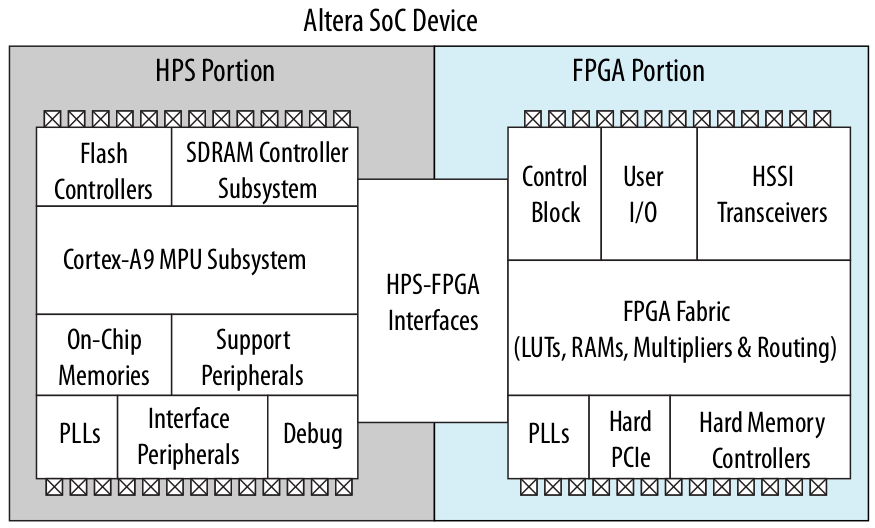
\includegraphics[width=10cm,keepaspectratio=true]{bilder/png/AlteraSoC}
\caption{Block diagram of an Altera Cyclone V SoC\cite[chapter 1]{AlteraHPS15}}
\label{fig:alterasocblocks}
\end{center}
\end{figure}
%FPGA Field Programmable Gate Array
\section{FPGA}
The FPGA portion of the Altera SoC is made for logic operations and high speed calculations, especially of matrices. Generally it can be said that everything which can be defined by the FPGA block layout can be implemented. Hence also interfaces like SPI or I$^2$C can be implemented in the FPGA. An FPGA consists of some main building blocks, which are described below.
\subsection{Logic Array Blocks (LAB)}
LABs are basic building blocks, each consisting of 10 adaptive logic modules (ALM). They are freely configurable to build up logic functions, arithmetic or register functions. A quarter of the LABs is configurable as memory (MLAB), which is described in chapter \ref{chap:embmem}. LABs can drive the own ALMs as well as the 20 ALMs of the adjacent LABs. The ALMs of one LAB can be driven by their own LAB and by DSP blocks using the direct link connection of the local interconnect. An ALM contains 4 registers, each having data, clock, clear, and synchronous load ports. The ALMs of the Cyclone V device can operate in 4 different operating modes\cite[chapter 1]{AlteraFPGA15}:
\begin{itemize}
\item Normal mode\\
In normal mode, up to 8 inputs from the local interconnect can be used to build up two functions with 4 inputs or one function with up to 6 inputs in one ALM. 
\item Extended LUT mode\\
In extended LUT mode, functions with 7 inputs can be implemented, if they fit into a template shown in figure \ref{fig:extendedlutfigure}. In HDLs, these functions are often designed as if/else-statements.
\begin{figure}[htbp]
\begin{center}
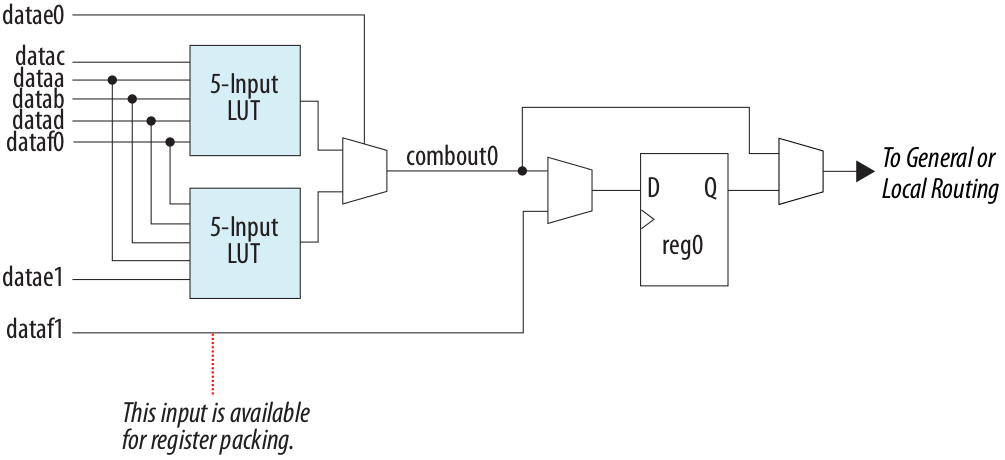
\includegraphics[width=10cm,keepaspectratio=true]{bilder/png/extendedlutfigure}
\caption{Template for functions in extended LUT mode\cite[chapter 1]{AlteraFPGA15}}
\label{fig:extendedlutfigure}
\end{center}
\end{figure}
\item Arithmetic mode\\
In the arithmetic mode, two dedicated full adders are available to perform pre-adder logic by the LUTs. Two additional functions with 4 inputs can be implemented, and the results of these functions can be added using the full adders.
\item Shared arithmetic mode\\
In the shared arithmetic mode, an adder with three inputs can be implemented. The ALM is configured with 4 input LUTs, with each LUT computing the sum of three inputs.
\end{itemize}
\subsection{Embedded Memory}
\label{chap:embmem}
A Cyclone V device has two different kinds of embedded memory: 10 kB blocks (called M10K) for providing memory for larger arrays, and MLABs with 640 bit memory for smaller memory arrays. MLABs are optimized for implementing shift registers used by DSPs. The embedded memory of the Cyclone V device supports different memory modes:
\begin{itemize}
\item Single-port RAM\\
The single-port RAM mode supports only one read or write operation at one specific time.
\item Simple dual-port RAM\\
In this mode, one read and one write operation can be done at the same time, if the read and write operation is done on different ports.
\item True dual-port RAM\\
In this mode, all combinations of read/write at two ports can be done. This includes two read operations, two write operations or one write and one read operation on two ports at different frequencies. This mode is only supported by M10K memory blocks.
\item Shift register\\
Logic cells and routing ressources for DSPs (like FIR, correlation functions, or pseudo random number generators) can be implemented in shift register mode. Memory blocks can be cascaded to implement larger shift registers.
\item ROM\\
An embedded memory block can be used as ROM as well. This is similar to the single-port mode, disabling the possibility for write operations. The data is loaded into the memory using .mif or .hex-files.
\item FIFOs\\
FIFO buffers can be implemented using either M10K or MLAB memory cells. For smaller FIFOs, MLABs are ideal for implementation, but mixed-width FIFOs are not supported using MLABs.
\end{itemize}
More information on embedded memory modes and clocking is available in \cite[chapter 2]{AlteraFPGA15}.
\subsection{Digital Signal Processing}
The Altera Cyclone V SoC contains some built-in DSP blocks for efficient signal processing. A block diagram of the used DSP architecture built is shown in figure \ref{fig:fpgadsp}.
\begin{figure}[htbp]
\begin{center}
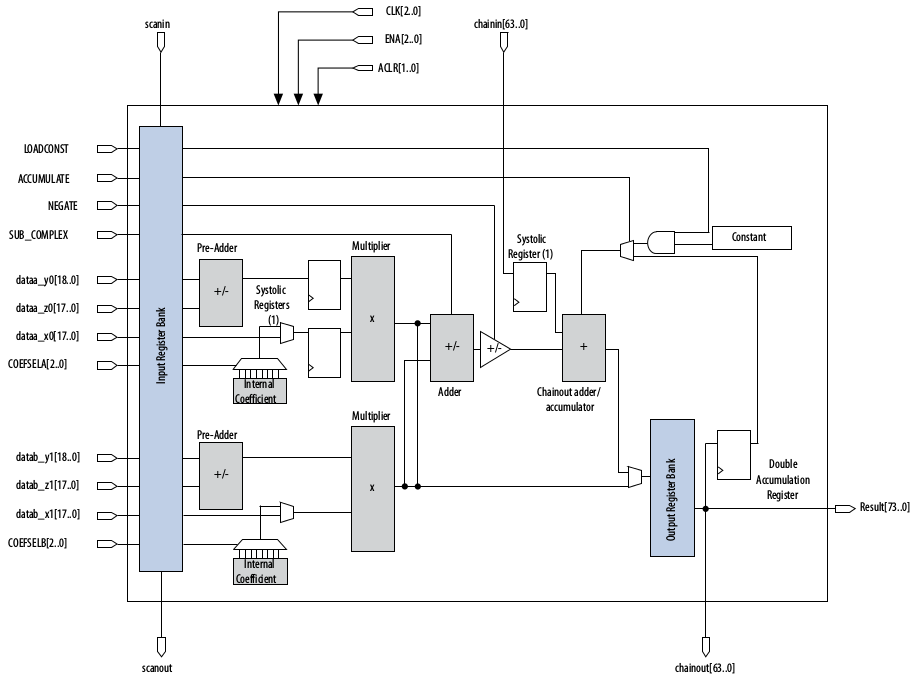
\includegraphics[width=15cm,keepaspectratio=true]{bilder/png/fpgadsp}
\caption{Cyclone V DSP architecture\cite[chapter 3]{AlteraFPGA15}}
\label{fig:fpgadsp}
\end{center}
\end{figure}
The DSP consists of following main components:
\begin{itemize}
\item Input register bank\\
The positive edge-triggered input register bank consists of data, dynamic control signals, and two sets of delay registers. The delay registers can be used to fulfill latency requirements.
\item Pre-adder\\
In each DSP block, there are two 19 bit pre-adders, which can be used either independently or combined as one 27 bit pre-adder.
\item Internal coefficient\\
For multiplications, the multiplicand can be given in two ways. It can be read from the dynamic input or the internal coefficient. This internal coefficient supports up to 8 different coefficients.
\item Multipliers\\
One reason for using DSPs is the high performance of calculating huge amounts of data, especially given in matrices. Due to this, each DSP block has two multipliers for performing many multiplications in parallel. The multipliers can be configured in following operation modes:
\begin{itemize}
\item 1 27$\times$27 multiplier
\item 2 18$\times$19 multipliers
\item 3 9$\times$9 multipliers
\end{itemize}
\item Adder\\
The adder can be used as one 64 bit adder, two 18$\times$19 adders or three 9$\times$9 adders, depending on the operational mode.
\item Accumulator and chainout adder\\
The accumulator supports double accumulation in the 64 bit mode and is neither available in the 18$\times$19 mode nor in the 9$\times$9 mode. The accumulation registers are set statically in the programming file. 
\item Systolic registers\\
The systolic registers are used to register the 18/19-bit inputs of the upper multiplier and to delay the chainout output to the next DSP block. It is used only in the systolic FIR mode and bypassed in all other modes. 
\item Output register bank
\end{itemize}
\subsubsection{DSP operation modes}
In this part, some important DSP operation modes of the built-in DSP block are described. Detailed block diagrams of the different operation modes can be found in \cite[chapter 3]{AlteraFPGA15}.
\paragraph{Independent multiplier mode}
In this mode, individual multiplication operations for general purpose multipliers are done. The following configurations can be used: 9$\times$9, 18$\times$18, 18$\times$19, 18$\times$25, 20$\times$24 and 27$\times$27.
\paragraph{Independent complex multiplier mode}
The DSP also supports multiplication of complex numbers. This is available for 18$\times$19 numbers and is done using the equation
\begin{equation}
(a+jb)\cdot (c+jd)=[(a\cdot c)-(b\cdot d)]+j[(a\cdot d)+(b\cdot d)].
\end{equation}
For the calculation, two DSP blocks are used, one for calculating the real part, the other one for the calculation of the imaginary part.
\paragraph{Systolic FIR mode}
FIR filters have an impulse response which goes to zero in finite time. In comparison to IIR filters, they have some useful properties:
\begin{itemize}
\item Stability: as the number of inputs is limited, also the ouput of the filter has a limited value.
\item No need for feedback.
\item Can be designed to have a linear phase.
\end{itemize}
Because of these properties, FIR filters are well suited, especially for phase-sensitive applications like data communications. For this reason, a dedicated FIR mode is built-in in the DSP blocks. The FIR filter output is calculated using the following formula:
\begin{equation}
y[n]=\sum_{i=1}^{k}c[i]x[n-i-1]\;.
\end{equation}
As the delay can become large with an increasing number of additions, a systolic form of the equation is used to overcome this delay. For this additional delay, elements are inserted to increase the calculation performance at the cost of increased latency. FIR calculations can be done using either 18 or 27 bit.
\subsection{Considerations regarding power}
It should be ensured that the read-enable signal is only set when necessary. When no read-during write is needed, the read-enable signal should be disabled. Due to this, read operations occur less often and the AC power consumption can be lowered significantly when this is applied to each memory block.\cite[chapter 1]{AlteraFPGA15} Generally, when using the system in a power-critical environment like in space, it should be noted that when using the FPGA, the overall power consumption is higher than when using only the HPS. Accordingly, the tradeoff between higher calculation speed for specific purposes and higher power consumption of the system should be compared.
%HPS Hard Processor System
\section{HPS}
One of the main parts of the Altera SoC is the hard processor system (HPS). It offers a microprocessor system for general purpose use. For procesing, a dual-core processor is used. A main task of the HPS is to connect to peripherals. Moreover, the connection to the FPGA portion is done and controlled using the HPS. The speed of the HPS does not only depend on the clock frequency of the MPU core, but also on cache speed and the speed of the data flow generating input for the MPU core. The main parts of the HPS, shown in figure \ref{fig:alterahpsblocks}, are described below.
\subsection{System interconnect}
The data exchange between different hardware blocks of the HPS is done via the interconnect system, consisting of the L3 main interconnect and the L4 bus system. Furthermore the L3 system has 3 major parts:
\begin{itemize}
\item L3 interconnect, with a data width of 64 bit. It is used to connect master blocks to slaves like the SDRAM controller subsystem, on-chip memories or the FPGA manager.
\item L3 master peripheral switch. This part has a data witdh of 32 bit and is used for memory-mastering peripherals.
\item L3 slave peripheral switch. Masters of the master peripheral switch and the interconnect use this block for interconnect. The data width is 32 bit. Furthermore the L3 slave peripheral switch has 5 different L4 buses.
\end{itemize}
While the master peripheral as well as the slave peripheral switch are fully connected crossbars, the L3 interconnect is partially connected. Therefore a data exchange is only possible for predefined block combinations. These can be found in \cite[chapter 7]{AlteraHPS15}.
\begin{figure}[htbp]
\begin{center}
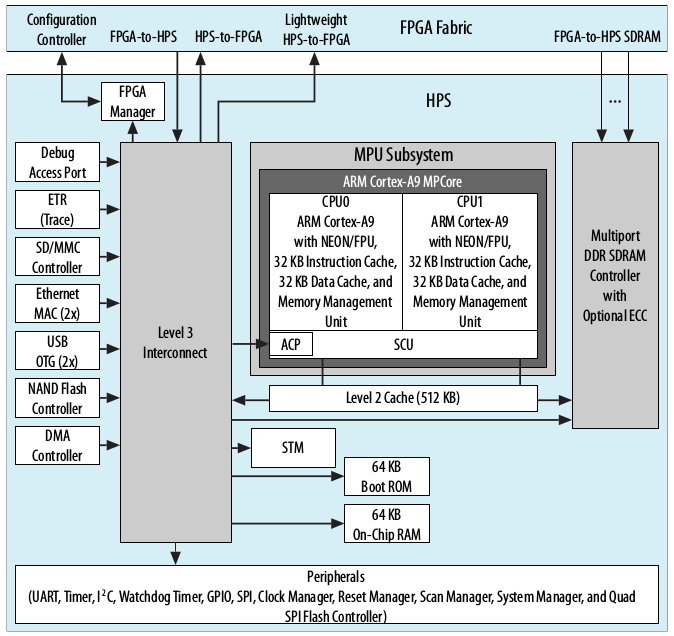
\includegraphics[width=15cm,keepaspectratio=true]{bilder/png/AlteraHPSneu}
\caption{Block diagram of an Altera Cyclone V HPS\cite{altcycvov15}}
\label{fig:alterahpsblocks}
\end{center}
\end{figure}
%MPU subsystem
\subsection{MPU subsystem}
The HPS consists mainly of a 32-bit dual-core ARM Cortex A9 microprocessor, with 32 kB instruction cache and 32 kB data cache for each processor core. The two caches are independent and therefore simultaneous loading  instructions and data. Each cache supports parity checking. The latency of loading data depends on the availability of the data. In case data and instructions are available in the L1 cache, the hit takes 1 clock cycle, if it is available in the L2 cache the best case is 6 cycles. If the data is not available in a cache, the latency varies depending on other operations. For this, a so called preload engine (PLE) is implemented. This hardware block allows the L2 cache to preload different memory regions defined by software control. Furthermore the endianess of the system can be configured.\\
In a shared system with multi-processing possibilities and a single data source, a hardware block to ensure coherency between processor cores and to ensure data consistency is needed. For this reason, a snoop control unit (SCU) is implemented. This unit manages the data traffic for all Cortex A9 processor cores and the memory system including the L2 cache. In case of a SMP configuration, also the data caches are maintained. Coherency of the instruction caches is not maintained in the SMP nor in the AMP configuration. Implementation details of the SCU can be found in \cite[chapter 9]{AlteraHPS15}.\\
For an efficient calculation of floating point operations, a FPU with full support of IEEE-754 half, full and double precision data is available, as well as convertion functionality between integer and floating point data types. For fast calculation of signal processing applications such as video and audio processing, an additional block called multimedia processing engine (MPE) is implemented. The MPE supports SIMD processing. The principle of SIMD is shown in figure \ref{fig:alterahpssimd}.
\begin{figure}[htbp]
\begin{center}
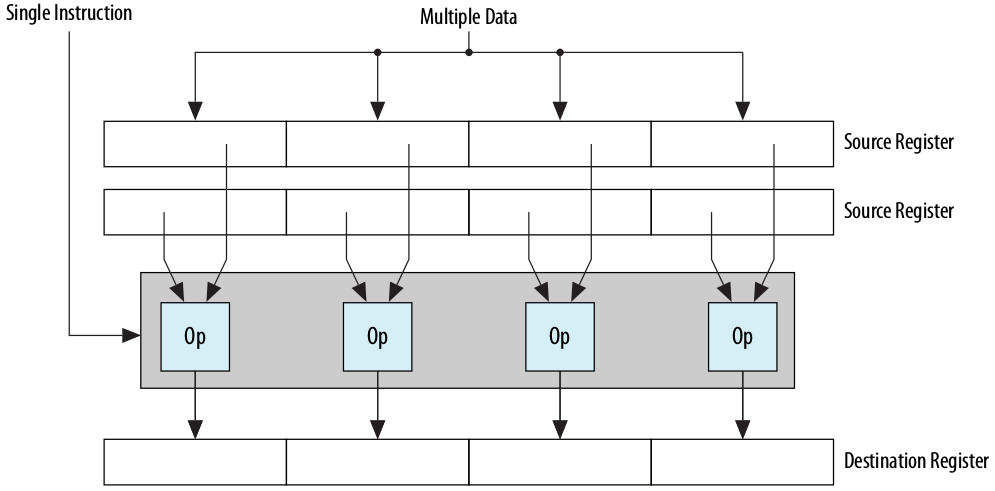
\includegraphics[width=12cm,keepaspectratio=true]{bilder/png/SIMD}
\caption{Principle of SIMD processing\cite[chapter 9]{AlteraHPS15}}
\label{fig:alterahpssimd}
\end{center}
\end{figure}
%SDRAM Controller Subsystem
\subsection{SDRAM controller subsystem}
The HPS SDRAM controller subsystem is used to access an external SDRAM memory with size of up to 4 GB for the following elements and interfaces:
\begin{itemize}
\item The MPU subsystem: dedicated 64-bit AXI interface.
\item The FPGA portion: the interface consists of 64-bit read data ports, 64-bit write data ports and command ports to build up three AXI interfaces or six Avalon-MM interfaces in total.
\item The L3 interconnect: dedicated 32-bit AXI interface.
\end{itemize}
Therefore this subsystem provides an interface between the HPS and the FPGA portion. The SDRAM controller can be subdivided into an MPFE and a single-port controller. While the single-port controller communicates with each external memory device, the MPFE provides several interfaces to the single-port controller through different FIFOs. As external memories, DDR2, DDR3 and LPDDR2 devices can be used. Implementation details of the SDRAM controller subsystem can be found in \cite[chapter 11]{AlteraHPS15}.
%SD/MMC-Controller
\subsection{SD/MMC-Controller}
As the internal memory of the Altera SoC has a very limited on-Chip memory, the storage of preloaders and operating systems for the HPS on external memory devices is very useful. For this reason, a SD/MMC controller for using SD and MMC flash cards as well as CE-ATA hard drives is implemented. The HPS has access to this controller with a 32-bit bus via the L3 interconnect. The SD/MMC-controller supports voltage levels of 3.3 V and, if it is supported by the card after power up, 1.8 V. It has to be noted that that kind of voltage switching is not supported by the controller itself but can be done using GPIO. Implementation details can be found in \cite[chapter 14]{AlteraHPS15}.
%System interconnect
%Clock manager
\subsection{Clock Manager}
In the HPS, different clocks organized in clock groups are used. Every clock is derived of the two main clocks \texttt{HPS\_CLK1} and \texttt{HPS\_CLK2} of the system. The clock generation of the HPS is done by the clock manager hardware block, shown in figure \ref{fig:hpsclockmanager}. 
\begin{figure}[htbp]
\begin{center}
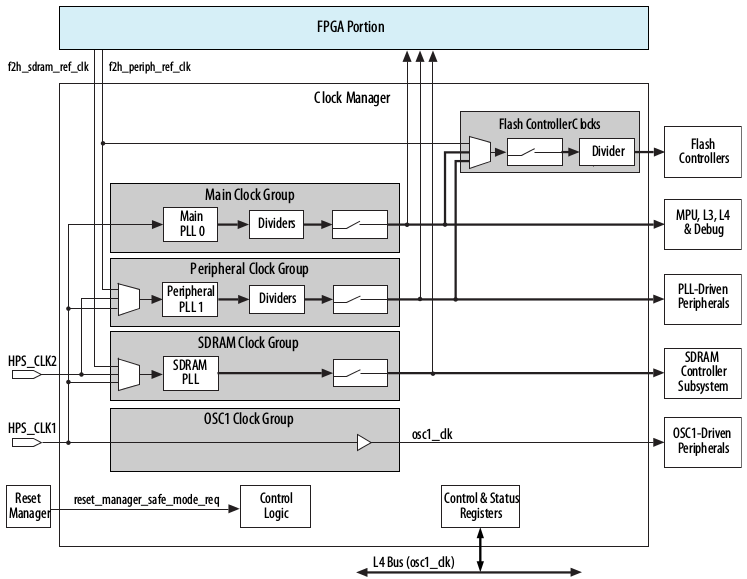
\includegraphics[width=15cm,keepaspectratio=true]{bilder/png/hpsclockmanager}
\caption{Clock generation of an Altera Cyclone V HPS\cite{altcycvov15}}
\label{fig:hpsclockmanager}
\end{center}
\end{figure}
A derivation of the different clocks is done using a PLL, where the frequency is set with a VCO. Dividers are used to lower the generated frequency. For generating clocks, three PLLs are available. The clock manager contains 4 different clock groups:
\begin{itemize}
\item OSC1 clock group\\
The OSC1 clock group has only one clock which is not divided and directly taken from the \texttt{HPS\_CLK1} as input for a PLL. It is used for OSC1-driven peripherals.
\item Main clock group\\
The PLL input of this group is derived of the \texttt{HPS\_CLK1}. It contains 5 dividers to generate different clocks for the MPU, SD/MMC-controller or, among others, the system interconnect.
\item Peripheral clock group\\
The peripheral clock group is used for clocking interfaces like USB, CAN and GPIO. The PLL can be sourced either from \texttt{HPS\_CLK1}, \texttt{HPS\_CLK2} or the \texttt{f2h\_periph\_ref\_clk} provided by the FPGA. The peripheral clock group has 5 dividers to provide 5 different clocks.
\item SDRAM clock group\\
The SDRAM clock group can use the  \texttt{HPS\_CLK1}, \texttt{HPS\_CLK2} or the \texttt{f2h\_sdram\_ref\_clk} clock provided by the FPGA for the SDRAM PLL.
\end{itemize}
A detailed description of the different clocks generated in the clock groups can be found in \cite[chapter 2]{AlteraHPS15}.
\subsubsection{Considerations on the used PLL}
The VCOs of the used PLLs have frequency stability up to $\newcommand*\rfrac[2]{{}^{#1}\!/_{#2}}\rfrac{+}{-}$20 percent of the used frequency and do not lose the PLL locking within this range. Thus when there is a need for changing the frequency more than 20 percent, a slow ramp up or down of the VCO is a possibility to change frequency without losing the lock. Another possibility, when e.g. lowering the frequency to the half, is to decrease the frequency by 20 percent for three times and divide it by 2.4 percent in a last step.
%System manager
\subsection{System Manager}
The system manager connects modules for system level functions like the DMA controller or the SD/MMC-controller. Furthermore it contains CSRs to monitor and control functions by software access. The system manager also contains information about boot configurations and defines which bootROM-code to execute. Detailed descriptions of how the system manager works and how the different controllers of the system manager are defined can be found in \cite[chapter 5]{AlteraHPS15}.
%FPGA manager
\subsection{FPGA Manager}
This module of the HPS is used to manage and configure the FPGA of the SoC. For this, 32 general-purpose input as well as 32 general-purpose output signals to the FPGA are available. Handshaking is also done using this block when booting the HPS from the FPGA portion. When the FPGA is in user mode, it offers registers for low latency communication between FPGA and HPS. The most important function of the FPGA manager is the configuration of the FPGA. When the FPGA is configured by the HPS, the only possibility to do this is using the FPGA manager.
%When the FPGA is in user mode it offers following registers for low latency communication between FPGA and HPS:
%\begin{itemize}
%\item \texttt{gpi}: general-purpose input register. The 32 input signals from the FPGA are read from this register.
%\item \texttt{gpo}: general-purpose output register. Output signals to the FPGA are written to this register.
%\item \texttt{misci}: boot handshaking input register. Those 2 signals are used by the bootROM code to determine if the preloader image stored in the FPGA should be used for the boot process.
%\end{itemize}
For more information about the implementation of the FPGA manager see \cite[chapter 5]{AlteraHPS15}.
%FPGA-HPS-Bridge
\subsection{HPS-FPGA-bridges}
Data exchange between FPGA and HPS is done using bridges. For this reason, three bridges are implemented in the Altera SoC:
\begin{itemize}
\item FPGA-to-HPS-bridge\\
Masters in the FPGA communicate with slaves in the HPS using this bridge. Peripherals and memory in the HPS can also be accessed when using the FPGA-to-HPS-bridge. While the bridge master interface (connected to the L3 intercconnect)  is fixed to 64 bit width, the bridge slave interface (connected to the FPGA) can be configured to 32 bit, 64 bit or 128 bit width. When the ECC option in the L2 cache is enabled, the width has to be 64 bit. 
\item HPS-to-FPGA-bridge\\
The HPS-to-FPGA bridge provides most masters of the HPS access to logic, peripherals and memory of the FPGA. The master interface is connected to the FPGA portion and has a configurable width of 32, 64 or 128 bit, on the other hand the width of the slave interface of the bridge is fixed to 64 bit. As the HPS-to-FPGA-bridge provides cross clocking, it can work independently and asynchronously to the HPS clock in any clock domain. 
\item Lightweight HPS-to-FPGA-bridge\\
This bridge is a HPS-to-FPGA-bridge with lower performance and a fixed master interface width as well as slave interface width of 32 bit. The lightweight HPS-to-FPGA-bridge can be used for low-bandwidth traffic and is useful for taking over some traffic, like accessing CSRs of soft peripherals, from the HPS-to-FPGA-bridge. The overall system performance can be increased significantly, using all bridges at optimal capacity usage.
\end{itemize}
For implementation details and a technical specification of the bridges see \cite[chapter 8]{AlteraHPS15}.
\section{Interfaces}
In this section the most important inferfaces of the Altera Cyclone V SoC are described.
\subsection{UART}
UART is a transmission protocol which was developed in the 1960s. UART is highly flexible in the sense that voltages, timing, error checking and flow control can be configured as the application needs. The commonly supported baud rates of UART are 600-921600 baud/s. As the history of UART is quite long, some different physical layer standards have been developed, such as RS232C or RS485. Due to this long development history, also many radiation hardened devices exist, like the Aeroflex DRS4485.\cite{aeroflex14}
\subsection{GPIO}
A GPIO is a digital interface which is made of pins with no dedicated usage. It is possible to configure them flexibly during runtime to act as input or output.
\begin{itemize}
\item When the pin is configured as input, it can read data from a digital circuit.
\item A binary signal can be sent to a digital circuit when the pin is configured as output.
\end{itemize}
GPIO-pins are available on most SoC and FPGA-devices, in some cases it is possible to configure every pin with no dedicated usage as GPIO-pin.\cite{kernelgpio15}
\subsection{I$^2$C}
The I$^2$C-bus was intentionally developed by Philips in the early 1980s to exchange information between ICs located on the same board. This bus is designed for synchronous transmission and is built up of ground, data and clock line. As advantages of this protocol, the clock reconstruction possibilities at the receiver have to be mentioned. Furthermore an arbitrary protocol guarantees that only one master exists at the same time.\cite{Wue06} I$^2$C defines communication modes as follows:
\begin{table}
\begin{center}
\begin{tabular}{|c||c|c|}
\hline
Mode & Maximum transmission speed & Direction\\
\hline\hline
standard mode & 100 kbit/s & bidirectional\\
\hline
full speed & 400 kbit/s & bidirectional\\
\hline
fast mode & 1 Mbit/s & bidirectional\\
\hline
high speed mode & 3.2 Mbit/s & bidirectional\\
\hline
ultra fast mode (UFm) & 5 Mbit/s & unidirectional\\
\hline
\end{tabular}
\caption{Speed grades of I$^2$C-transmissions\cite{I2Cspeed}}
\label{tab:rsstates}
\end{center}
\end{table}
As the I$^2$C-bus is inteded to exchange data between ICs, the packet size is small. This leads to the fact that high accuracy of the clock is not needed for most applications.\cite{I2Cspeed} The I$^2$C-bus was intentionally designed for 5 V reference voltage. With the release of the specification I$^2$C-2.0, the bus got also the possibility to operate with 2 V references.\cite{I2Cvoltage}\\
More information can be found in the I$^2$C-specification in \cite{I2Cspec}.
\subsection{CAN}
The CAN-bus was developed by Bosch in the early 1980s as serial communication protocol for motorized vehicles. In 1994, it became the international standard ISO 11898. The protocol is able to handle bitrates up to 1 Mbit/s and has multi-master capability. That means that different bus members can have master state at different times. CAN is able to handle reference voltages of 5 V and 3.3 V.\cite{Corrig2008} The CAN-bus uses two signaling lines for communication. As CAN is designed as real time control protocol with a high level of security, it has some important features beside others\cite{boschcan91}:
\begin{itemize}
\item message priorization,
\item guaranteed latency times,
\item different error detection capabilities, and
\item autonomous switching off of defect nodes.
\end{itemize}
The specification of CAN can be found in \cite{boschcan91}, an even more detailed description in \cite{nxpcan98}.
\subsection {SPI}
The serial peripheral interface (SPI) was introduced by Motorola as bus standard for synchronous full duplex operation. It is built up as master/slave system. The initialization of a data transfer is always done by the master, but data can be sent in both directions. SPI communication is done with 4 signals. In fact, SPI is a very simple communication bus with no built in acknowledgement mechanism and no flow control. If these are needed, they have to be implemented in additional hardware around or by communication protocols. SPI offers high data rates up to several Mbit/s, with a high potential in single master single slave configurations.\cite{SPI02}
\subsection{USB}
The Universal Serial Bus (USB) is a serial communication bus with a speed up to 4 Gbit/s. Each bus is controlled by one host and can have up to 127 slaves, which are connected in a star topology. USB uses 4 wires, of which two are transferring data using a NRZI encoding scheme, the other two have a DC power of 5 V. This voltage is one of the main benefits of USB. Devices connected to an USB bus do not have to have external power supply if the bus is serving enough energy to power the device. A detailed description how USB works can be found in \cite{Pea10}. The full USB specification can be found at \cite{USB16}.
\section{Booting}
For booting, three different configuration options are possible:\cite[chapter A]{AlteraHPS15}
\begin{itemize}
\item The HPS preloader and the FPGA configuration are independent. In this case, the FPGA configuration image is loaded from an external source, and the HPS preloader is also located externally.
\item The HPS boots and the FPGA is configured after this by the HPS. The HPS preloader is loaded from an external memory. After the boot of the HPS, the FPGA is reset and a configuration image from a flash memory or a communication interface is loaded by the HPS to the FPGA.
\item The FPGA is configured and the HPS boots from the FPGA portion. For this, the FPGA configuration image is loaded from an external source. The FPGA is configured and contains a preloader image for the HPS. When using this initialization option, the HPS should not be released from reset state until the FPGA configuration is completed. After the HPS release, the HPS preloader image is executed by the BootROM over the FPGA-HPS-bridge.
\end{itemize}
When the SoC is booted from the HPS, the boot flow shown in figure \ref{fig:bootstages} is used.
\begin{figure}[htbp]
\begin{center}
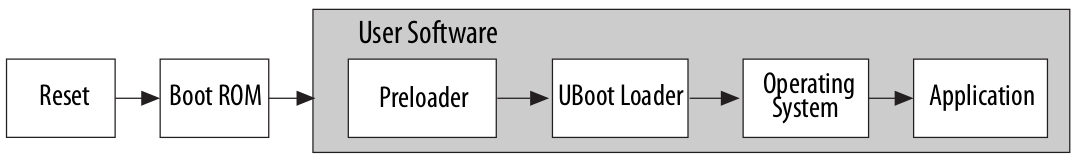
\includegraphics[width=13cm,keepaspectratio=true]{bilder/png/bootstages}
\caption{Boot steps of an Altera Cyclone V SoC\cite[chapter A]{AlteraHPS15}}
\label{fig:bootstages}
\end{center}
\end{figure}
\subsection{Reset}
\begin{itemize}
\item Cold reset\\
In case of a cold reset, all registers are initialized and the HPS starts executing the BootROM code located at the reset exception address. A cold reset is done whenever the device is booted after a full shutdown.
\item Warm reset\\
In case of a warm reset, some register contents are preserved. In addition, the device has the ability to execute a preloader located in the on-chip RAM.
\end{itemize}
\subsection{Boot-ROM}
The boot-ROM is located in the on-chip ROM and performs all actions needed for a basic initialization of the system. It determines the boot source, selected with the \texttt{BSEL}-pins, and configures the main PLL clock rate using the \texttt{CSEL}-pins. Furthermore the flash controller is set to default settings. After initialization, the boot-ROM jumps to the preloader. Depending on the location of the preloader, the first 4 kB of the on-chip RAM are used. When the preloader image is located on a flash device, this memory is reserved as working space for the HPS, otherwise it can be used for user purposes. It has to be noted that the Boot-ROM is always executed on CPU core 0. After the Boot-ROM has switched the control to the user software (the preloader), the access to the Boot-ROM is disabled.
\subsubsection{Booting from SD/MMC flash devices}
If the preloader image is stored on a flash device as shown in figure \ref{fig:sdboot}, the first 512 byte of the storage are used as MBR where the start addresses and sizes of the boot images on the device are stored. The images themselves are stored in a raw partition with no file system (shown as partition A2). As the on-chip RAM-size is limited to 64 kB and 4 kB are used as working memory (stack, ...), the preloader image has to have a maximum size of 60 kB. In case of a failure of the flash device, the Boot-ROM checks the FPGA portion for a bootable fallback image. 
\begin{figure}[htbp]
\begin{center}
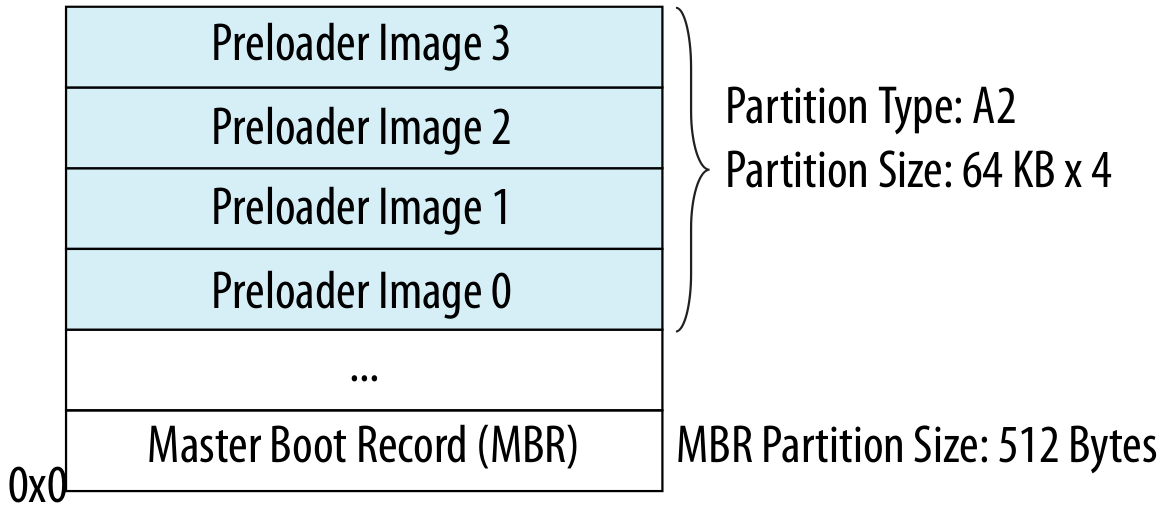
\includegraphics[width=8cm,keepaspectratio=true]{bilder/png/sdboot}
\caption{SD/MMC boot image layouts\cite[chapter A]{AlteraHPS15}}
\label{fig:sdboot}
\end{center}
\end{figure}
\subsection{Preloader}
The preloader is the first stage of the user software. Therefore the functionality of the preloader image is given by the user. Typical functions include the initialization of interfaces for booting the next software stage and the SDRAM interface. Furthermore the I/O-pins can be configured. The next software stage can be loaded from any interface available to the HPS and, after initialization of the SDRAM, is not limited to 60 kB as it is for the on-chip ROM.
\subsection{UBoot-Loader}
UBoot is a universal bootloader for a variety of devices, which are made for embedded systems. It was invented by DENX in 1999 and is available under the GPL. UBoot can be configured using a command line interface, the configuration can be safed to flash devices. Typically the UBoot-loader sets up the device tree, loads the operating system kernel and hands over the user software control to the kernel.
\subsection{Operating System}
Generally each operating system can be loaded by the HPS as long as some requirements are fulfilled. The boot flow needs to have the ability to be configured for the HPS. For this, beside others, drivers and a compiler for the ARM processor are required. Due to the fact that all requirements are fulfilled by Linux and the use is free of charge, Linux is recommended by the Altera corporation.